%%% -*-LaTeX-*-

\chapter{Background}
\label{cha:background}

An important concern in engineering blood-contacting devices is the
interaction between blood and artificial materials. Artificial devices
are commonly used to treat cardiovascular diseases, and they should
not trigger immune responses in the bloodstream. But materials
currently in use are not sufficiently blood-compatible and patients
with a blood-contacting device must take systemic anti\-coagulants to
reduce the risks of thrombosis and embolism
\cite{Ratner1993,Ratner2007,Oprea13}. The goal of the work presented
below is to model the mechanism by which platelets interact with a
reactive surface, and how these interactions activate platelets to
facilitate blood clotting.

This background chapter first summarizes the mechanisms of platelet
activation and their importance in blood clotting in section
\ref{sec:overview-clotting}. Then section \ref{sec:priming-project}
covers the relevance of platelet activation to the bio-materials
engineering problem of hemocompatibility. This section also presents
research from a biomedical engineering group at Utah led by Vladimir
Hlady that shows that platelets can be primed by interactions with a
reactive surface. Finally section \ref{sec:exist-cell-roll} reviews
existing models of leukocytes and platelets rolling along reactive
surfaces.

\section{Overview of the clotting pathway}
\label{sec:overview-clotting}

\begin{figure}
  \centering
  % \documentclass{article}
% \usepackage{tikz}
% \usetikzlibrary{backgrounds,fit,positioning}

% \begin{document}

\begin{tikzpicture}[
  node text/.style={
    align=center,
    draw, very thick,
    fill=white,
    rounded corners,
    inner xsep=10pt,
    inner ysep=7pt,
    minimum height=13mm,
  },
  connect/.style={shorten <=5pt, shorten >=5pt, thick},
  background/.style={rounded corners, inner xsep=10pt, inner ysep=10pt, draw, dashed,
    thick},
  ]
  
  \node[node text] (roll)
  {\begin{minipage}{.5\linewidth}
      \underline{Rolling}
      \begin{itemize}
        \setlength\itemsep{-.3em}
      \item transient contacts
      \item hydrodynamic vs. bond forces
      \item fast receptors trigger intracellular pathways
      \end{itemize}
    \end{minipage}
  };
  \node[node text] (actv) [below=of roll]
  {\begin{minipage}{.5\linewidth}
      \underline{Activation}
      \begin{itemize}
        \setlength\itemsep{-.3em}
      \item intracellular signaling
      \item release soluble agonists
      \item activate integrins for aggregation
      \end{itemize}
    \end{minipage}
  }
  edge [<-, connect] (roll);
  \node[node text] (aggr) [below=of actv]
  {\begin{minipage}{.5\linewidth}
      \underline{Aggregation}
      \begin{itemize}
        \setlength\itemsep{-.3em}
      \item cohesion among platelets
      \item adhesion to vessel wall
      \end{itemize}
    \end{minipage}
  }
  edge [<-, connect] (actv);
  \node[node text] (thrb) [below=2cm of aggr]
  {\begin{minipage}{.5\linewidth}
      \underline{Thrombin Formation}
      \begin{itemize}
        \setlength\itemsep{-.3em}
      \item plasma-phase reactions
      \item many coagulation factors involved
      \item prothrombin converted to thrombin
      \end{itemize}
    \end{minipage}
  }
  edge [<-, thick, shorten <=28pt, shorten >= 15pt] (aggr);
  \node[node text] (fibr) [below=of thrb]
  {\begin{minipage}{.5\linewidth}
      \underline{Fibrin Gelation}
      \begin{itemize}
        \setlength\itemsep{-.3em}
      \item thrombin converts fibrinogen to fibrin
      \item stabilize the clot
      \end{itemize}
    \end{minipage}
  }
  edge [<-, connect] (thrb);

  \begin{scope}[on background layer]
    \node [fill=lightgray, fit=(roll) (aggr), background,
    label=above:\textbf{Activation and Aggregation}] {};
    \node [fill=gray, fit=(thrb) (fibr), background,
    label=above:\textbf{Coagulation}] {};
  \end{scope}
\end{tikzpicture}
% \end{document}


  \caption{Summary of the major processes in the clotting pathway.}
  \label{fig:clot-path}
\end{figure}

There are two major processes in the blood clotting pathway: platelet
activation and coagulation. The dynamics of blood clotting are complex
and do not proceed in a linear fashion, and so the major processes of
activation and coagulation occur in parallel and feed back on each
other in complex ways. Nonetheless, it is convenient to describe in a
linear progression as sketched in Figure
\ref{fig:clot-path}. Platelets in the bloodstream activate in response
to binding to immobilized agonists on the vessel wall or soluble
agonists dissolved in the blood plasma, and upon activation platelets
begin clot formation and adhesion to the vessel wall.

As activated platelets begin to aggregate, extracellular chemical
reactions begin to occur both in the blood and on platelet surfaces,
ultimately resulting in the production of thrombin and the formation
of a fibrin gel. Coagulation refers specifically to the two processes
of thrombin generation and fibrin gelation \cite{Fogelson2015}. While
coagulation is important in facilitating the growth of clots and
stabilizing existing clots, it is not relevant in our model or in
Dr. Hlady's experiments. The platelet priming experiments use
anticoagulated blood, that is thrombin is inactivated and functionally
removed from the system.

Platelet activation is initiated by intracellular chemical
pathways. When platelet receptors bind with agonists, the receptors
trigger activation pathways which result in a suite of activation
responses: degranulation (i.e. release of ADP and other soluble
agonists), thromboxane A2 (TxA2) synthesis, activation and recruitment
of \ITA{IIb}\ITB{3} receptors, exposure of phosphatidylserine (PS),
and---after adhesion to a vessel wall---platelet spreading
\cite{Bye2016}.

\subsection{Platelet adhesion to an injury and aggregate formation}
\label{sec:platelet-adhesion}

In order for a platelet aggregate to form on the vessel wall,
platelets must adhere to the vessel wall and cohere to other
platelets. In normal hemostasis, platelets adhere to the vessel wall
by binding to the surface-immobilized proteins, collagen---which is
embedded in the sub-endothelial matrix---or von Willebrand Factor
(vWF)---which can either bind to exposed collagen, or is expressed by
endothelial cells when they activate \cite{Fogelson2015}. Platelets in
the blood roll along these proteins using fast-forming and
fast-breaking bonds, and these contacts trigger activation pathways
within the platelet. As a result of platelet activation, intracellular
signaling pathways activate integrin receptors on the platelet
surface, which mediate stable and long lasting bonds with vWF and
collagen \cite{Bye2016,Li2010,Fogelson2015,Qiu2015}. Figure
\ref{fig:transient-binding} shows a platelet transiently binding to
vWF which itself is adhered to endothelial cells lining the blood
vessel wall. This is just one example of a transient contact between
a platelet and an agonist-coated wall; platelets can also bind to
collagen and fibrinogen immobilized on a surface through different
receptors. 

\begin{figure}
  \centering
  \includegraphics[width=0.6\textwidth]{transient-binding}
  \caption[An example of transient platelet binding to vWF through
  GP1b.]{An example of transient platelet binding to vWF through
    GP1b. When GP1b is bound to vWF, it initiates intracellular
    signaling pathways resulting in platelet activation, and in
    particular activation of \ITA{IIb}\ITB{3} which can mediate stable
    adhesion.}
  \label{fig:transient-binding}
\end{figure}

Platelets constitutively express separate fast receptors for vWF and
collagen. The receptor GP1b binds to vWF molecules, and GPVI binds to
collagen. These receptors have fast binding and unbinding kinetics,
and are therefore able to form bonds with their surface-immobilized
ligands while the platelet moves past the reactive surface. When these
bonds form and stretch beyond their rest length, they exert a
force in opposition to the flow and slow the platelet down. Therefore
the motion of a platelet along a wall with immobilized agonists is a
function of the biochemical interactions of receptors and ligands as
well as the fluid forces exerted on the platelet.
		
These receptors are more than simple physical links between the
platelet and surface. When they bind with a ligand, they initiate
intracellular signaling cascades that trigger the release of
intracellular calcium and activate phosphatidylinositide-3-kinase
(PI3K) which are two crucial signaling molecules in the platelet
activation pathway \cite{Bye2016,Du2007,Senis2014}. These activation
signals ultimately terminate in a suite of responses that are
collectively called platelet activation. The responses include granule
secretion, TxA2 synthesis, cytoskeletal rearrangements, and activation
of the receptors \ITA{IIb}\ITB{3} and \ITA{2}\ITB{1}. These receptors
mediate firm adhesion of the platelet to vWF and collagen,
respectively. They are constitutively expressed on the surface of the
platelet, but on inactive platelets they exist mostly in their
low-affinity conformation and undergo a conformational change to their
high-affinity conformation after platelet activation
\cite{Qiu2015,Shattil1998,Shattil2010}.

\subsection{Secondary activation and platelet cohesion}
\label{sec:second-wave-activ}

An important result of platelet activation is the release of secondary
mediators of platelet activation TxA2 and ADP \cite{Bye2016}. These
are soluble platelet agonists which enter the blood and activate
platelets in the bulk flow, forming a positive feedback loop where
activated platelets release chemical signals that trigger more
platelets to activate. Activated platelets can then be recruited to
the growing clot by either binding to an agonist adhered to the wall,
or by cohering to an existing platelet aggregate.

Cohesion among platelets is mediated by vWF and fibrinogen---the
precursor to fibrin monomers \cite{Fogelson2015}. As mentioned before,
vWF binds with the GP1b and active \ITA{IIb}\ITB{3} receptors on the
platelet surface, and fibrinogen binds with active
\ITA{IIb}\ITB{3}. Both of these molecules circulate within the blood
plasma, and activated platelets can capture them from the blood,
immobilizing them on the platelet surface. When bound to the surface
of one platelet, these molecules act as a cross-bridge to which other
platelets within the blood can cohere.

\section{Description of the priming project}
\label{sec:priming-project}

Treatment of cardiovascular diseases often involves implanting medical
devices into the blood stream. For example, stents (an expandable
solid mesh) are often used to treat stenotic (i.e. blocked or impeded)
arteries. However, the introduction of a foreign material into the
blood stream will cause thrombosis unless the material is treated
somehow, and while these devices have been effective in treating
disease they still have negative side effects. For example, patients
with these implanted devices still must be placed on anticoagulants,
as they have a higher risk of a thrombotic event even when the device
is functional and surgery is successful \cite{Cannegieter1994}.

Most hemocompatibility studies focus on local interactions and effects
of artificial biomaterial on platelets. However recent work
\cite{Corum2011,Corum2012} carried out by Dr. Hlady's group has shown
that non-local effects are also important in understanding platelet
interactions with implanted bio-materials. In particular, while
platelet interactions with immobilized agonists may not cause the
platelets to adhere at the site of interaction, these interactions
nonetheless prime platelets for downstream adhesion and full
activation.

\begin{figure}
  \centering
  \begin{tikzpicture}[scale=.65]
  \tikzstyle{every node}=[font=\small]
  \pgftext{\includegraphics[width=\textwidth]{blood-vessel}}
  \draw[very thick, ->] (-3, 2.6) -- node[fill=white] {flow direction} +(5,.35);
  \draw[thick, ->] (-3.5, -3.5) node[below] {Native vessel} -- ++(0, 1);
  \draw[thick, ->] (1, -3.3) node [below] {Artificial vessel} -- ++(0, 1);
  \draw[thick, ->] (-1, -4) node[below] {Anastomoses} .. controls (-1, -2) .. +(-1.4, 3);
  \draw[thick, ->] (-.8, -4) .. controls (-.8, -2) and (0, -1) .. +(2.55, 3.5);
\end{tikzpicture}

  \caption[Cross-section of a blood vessel with a vascular
  graft]{Cross-section of a blood vessel with a vascular graft. There
    are two anastomotic regions at either end of the graft where
    artificial material is joined to native tissue.}
  \label{fig:blood-vessel}
\end{figure}

One example of this is a vascular graft, shown in Figure
\ref{fig:blood-vessel}. At either end of the implanted device, native
tissue must be joined with artificial material. At these points along
the vessel wall the tissue is inflamed and stenosed, which could
expose platelet agonists on the surface of the wall. Additionally the
increased shear rate in the stenotic regions could act to prime
platelets through a phenomenon known as shear-induced platelet
activation \cite{Fogelson2015,Kroll96,Shankaran2003}. Therefore while
platelets may not bind to a single inflamed region of the vessel, the
upstream region can prime platelets for adhesion, and then more
readily bind to the downstream inflamed region.

In order to investigate non-local effects of priming, Dr. Hlady's
group has designed a microfluidic assay with two regions printed with
platelet agonists (see Figure \ref{fig:flow-chamber})
\cite{Corum2012}. The upstream agonist region is called the priming
region, and the downstream region with agonist is called the capture
region. While these two regions have different names, there is no
chemical difference between them, the only difference is in their
locations in the flow chamber.

In the priming region, platelets close to the agonist-printed surface
of the flow chamber may have transient contacts with the agonist,
initiating activation pathways within the platelet. Some platelets may
firmly adhere in this priming region, but many will not and instead
will reenter the flow and get washed downstream to the capture
region. Once they reach the capture region, the platelets which
contacted the agonist in the priming region will have more active
integrin on their surfaces \cite{Corum2012}, more phosphatidylserine
exposed (unpublished data), and probably heightened levels of
intracellular activating chemicals like Ca$^{++}$. That is, they will
be primed to adhere with the capture region, and therefore adhere with
a greater frequency than unprimed platelets.

\begin{figure}
  \centering
  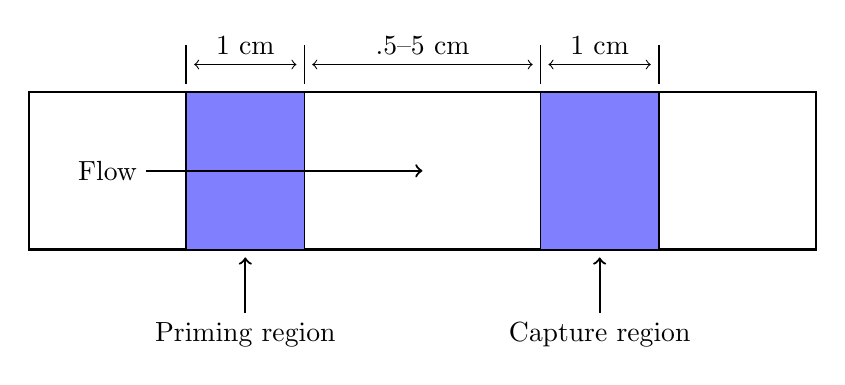
\begin{tikzpicture}
  \draw[thick] (-5, -1) rectangle (5, 1);
  \filldraw[semithick, fill=blue!50] (-3, -1) rectangle (-1.5, 1);
  \filldraw[semithick, fill=blue!50] (1.5, -1) rectangle (3, 1);
  \draw[thick, ->] (-4, 0) node[fill=white] {Flow} -- (0, 0);
  \draw[thick, ->] (-2.25, -1.8) node[below] {Priming region} -- ++(0, .7);
  \draw[thick, ->] (2.25, -1.8) node[below] {Capture region} -- ++(0,
  .7);
  \draw[semithick] (-3, 1.1) -- +(0, .5);
  \draw[semithick] (-1.5, 1.1) -- +(0, .5);
  \draw[semithick] (1.5, 1.1) -- +(0, .5);
  \draw[semithick] (3, 1.1) -- +(0, .5);
  \draw[<->] (-2.9, 1.35) -- node[midway, above] {1 cm} +(1.3, 0);
  \draw[<->] (1.6, 1.35) -- node[midway, above] {1 cm} +(1.3, 0);
  \draw[<->] (-1.4, 1.35) -- node[midway, above] {$.5$--$5$ cm}(1.4,
  1.35);
\end{tikzpicture}

  \caption[The microfluidic chambers used in Dr. Hlady's priming
  experiments.]{Schematic of the microfluidic chambers used in
    Dr. Hlady's priming experiments. Blood is perfused from left to
    right over the priming and capture regions. Either immobilized
    agonist or a nonreactive control is printed in the priming and
    capture regions}
  \label{fig:flow-chamber}
\end{figure}

In previous research, Dr. Hlady's group has found that all 3
immobilized platelet agonists tested (vWF, collagen, and fibrinogen)
in the upstream region increased adhesion of platelets in the capture
region relative to a nonreactive control
\cite{Corum2012,Eichinger2016}. Recent unpublished work has shown
similar results when the upstream agonist printing was replaced by a
stenotic region with higher wall shear rates. In addition, flow
cytometry has revealed that platelets in blood which has been perfused
over surface-immobilized agonists express higher concentrations of
several different activation markers \cite{Corum2012,Eichinger2016}.

In addition to the adhesion and flow cytometry experiments,
Dr. Hlady's group is studying the effect of priming on the
rolling behavior of platelets over immobilized agonists. In this set
of experiments, a camera captures video of platelets rolling along the
capture region, and from this data they extract average platelet
rolling velocities, average step sizes, and dwell times of rolling
platelets. The step size is the length a platelet travels in the
direction of flow in between binding to the wall. The dwell time is
the length of time a platelet spends transiently attached to the wall
in between steps.

While flow cytometry is a useful tool to precisely measure quantities
of active receptors and other proteins, platelets must be incubated
with marker chemicals for 20 minutes before measurement, making the
measurements of platelet activation markers temporally imprecise. On
the other hand, the behavior of rolling platelets can be observed in
real time, but the relationship between rolling behavior and platelet
activation state is not clear. The model presented below and the
planned future work focuses on quantitatively connecting parameters of
platelet receptor binding and unbinding to rolling behavior. The rest
of this chapter lays out a brief review of published mathematical
models of cell rolling in blood. Chapter \ref{cha:model} describes a
new model of cell rolling which includes individual receptor and bond
dynamics, but is simpler than existing models which treat individual
bonds separately. Chapter \ref{cha:results} explores the behavior of
the model under simplified conditions, and demonstrates that the model
predicts different rolling behavior for different platelet activation
states. Finally chapter \ref{cha:future-work} discusses extensions of the
basic model which incorporate more physical and biological complexity.

\section{Existing cell rolling models}
\label{sec:exist-cell-roll}

A large body of work has been published on the subject of cell rolling
and adhesion, including mathematical models of cell rolling
\cite{Pospieszalska2009,Sundd2011}. However most of the modeling work
focuses on leukocyte rolling on an agonist-coated surface. Modeling of
platelet rolling is less common.

The existing rolling models cover a wide range of assumptions and vary
from simple and highly idealized to detailed and complex. The simplest
rolling models often treat cells as a continuum and only reproduce
population-wide averages of rolling velocity of rolling cells, and
greatly simplify hydrodynamic and chemical forces. At the other end of
the spectrum, the most complex models use much more detailed
hydrodynamic and chemical forces, often explicitly tracking individual
receptors and ligands on the surface of the cell and the surface of
the vessel wall, and modeling the rolling behavior of individual cells
as a stochastic process. 

The data Dr. Hlady's group is collecting cannot be captured in a
deterministic and continuous model of bond formation, so a model with
stochastic bond formation that captures rolling behavior of individual
platelets is the best fit for the available data. One common family of
rolling models are the adhesive dynamics models, which model the
formation and breaking of bonds as stochastic events, and these models
lie on the more complex end of the spectrum of rolling models.

\subsection{Adhesive dynamics models}
\label{sec:adhesive-dynamics}

Adhesive dynamics (AD) is a common modeling framework for
leukocytes. Hammer \& Apte \cite{Hammer1992} published the first
adhesive dynamics model in 1992, and this model provides a good
example to describe the AD models in general. It is convenient to view
more recent models as modifications of this fundamental model. They
model a leukocyte as a rigid sphere, with rigid microvilli protruding
normally from the surface of the cell. Receptors are located only at
the tips of these microvilli (multiple receptors can occupy a single
microvillus), and can bind to ligand binding sites which are uniformly
distributed along a flat wall (Figure \ref{fig:ad-geom}). The
positions and bound state of each receptor is tracked throughout the
simulation. Binding and unbinding of receptors is modeled by a
stochastic process with length-dependent rates given by the Dembo
model \cite{Dembo1988}:
\begin{align}
  \label{eq:dembo-on}
  k_\tn{on} \left(L_\tn{sep}\right)
  &= k_\tn{on}^0 \exp \left( -\frac{\sigma_\tn{ts} (L_\tn{sep} -
    \lambda)^2}{2\boltzmann \temp} \right) \\
  \label{eq:dembo-off}
  k_\tn{off} \left(L_\tn{sep}\right)
  &= k_\tn{off}^0 \exp \left( \frac{(\sigma - \sigma_\tn{ts})
    (L_\tn{sep} - \lambda)^2}{2 \boltzmann \temp} \right).
\end{align}
where $\lambda$ is the equilibrium separation distance,
$\boltzmann\temp$ is the thermal energy, $\sigma$ is the spring
constant, and $\sigma_\tn{ts}$ is the transition state spring
constant.

\begin{figure}
  \centering
  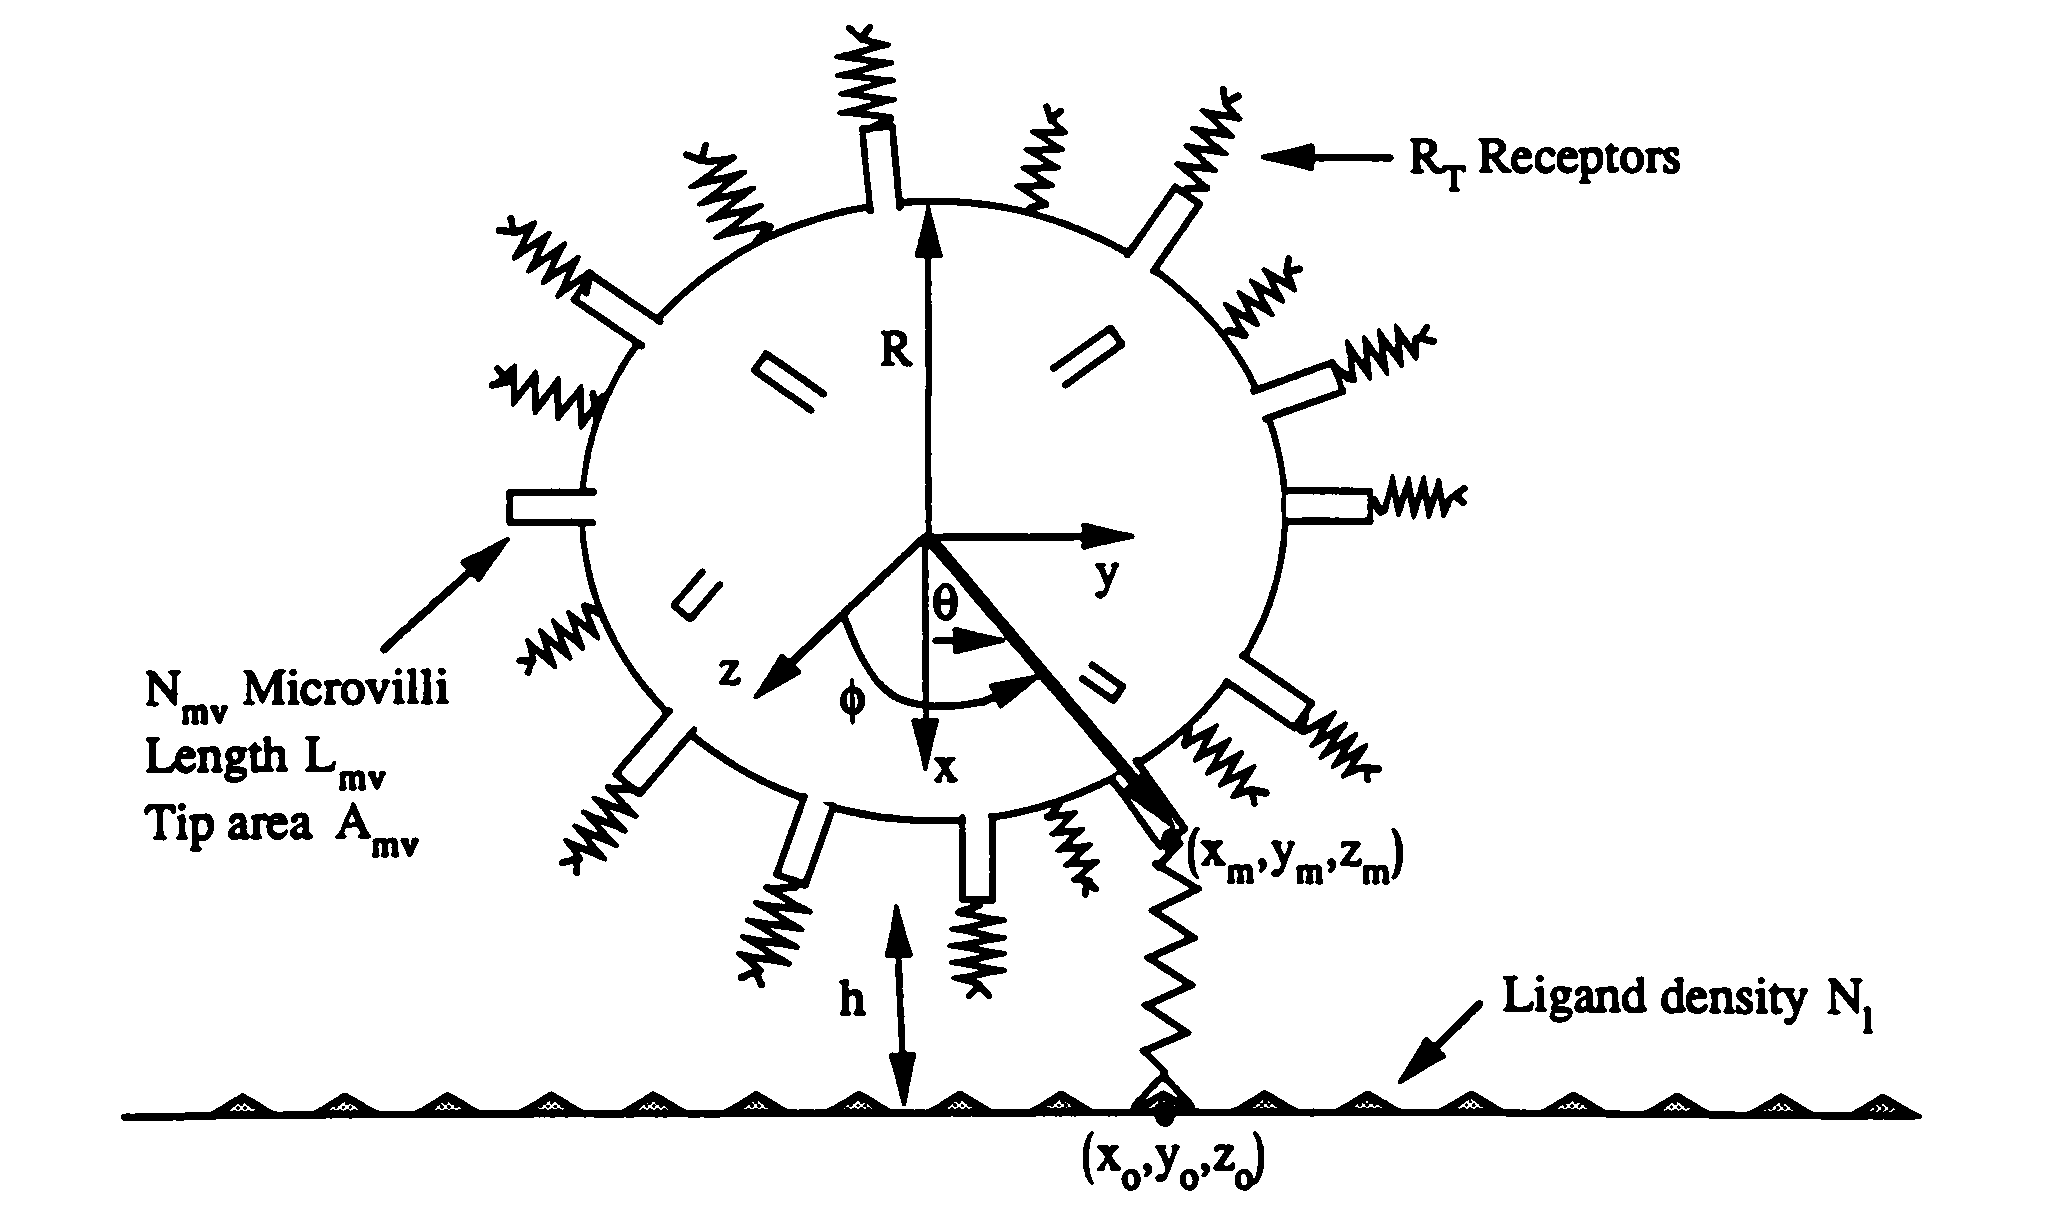
\includegraphics[width=0.75\textwidth]{hammer92scr.jpg}
  \caption[Model geometry in the adhesive dynamics model of Hammer \&
  Apte.]{Model geometry in the adhesive dynamics model of Hammer \&
    Apte. The leukocyte is moving near a ligand-covered wall, and
    receptors are clustered on the tips of microvilli protruding from
    the cell. Figure is reproduced from \cite{Hammer1992}}
  \label{fig:ad-geom}
\end{figure}

Force balance between hydrodynamic drag forces, bond forces, and
colloidal forces defines the movement of the leukocyte. The
hydrodynamic forces are found by assuming that the fluid surrounding
the leukocyte is a Newtonian fluid with $\Reynolds = 0$ at the
relevant length and time scales of the problem, and that the fluid is
moving in a shear flow. Under these assumptions, there is a linear
relationship between the drag force $\forceVec_\tn{drag}$ on the cell and the
velocity $\velVec$: $\forceVec_\tn{drag} = \resMatrix \velVec$. The colloidal
forces on the cell are split up into 4 different forces: van der Waals
forces, gravitational body force, electrostatic force, and steric
stabilization force.

\subsubsection{Extensions of AD}
\label{sec:extensions-ad}

Many extensions and adaptations of the AD model have been made since
its publication. In \cite{Bhatia2003}, Bhatia, King, and Hammer model
leukocyte rolling with two classes of receptors: fast binding and
unbinding selectins (P-selectin--sLe\textsuperscript{x}), and slow
binding and unbinding integrins (\ITB{2}-integrin--ICAM-1). They plot
the effect of modulating the selectin and integrin ligand surface
densities by creating state diagrams which characterize the cell
rolling behavior in different regions of this 2D parameter space. They
showed the effect of neutrophil activation on these state diagrams by
increasing the $k_\tn{on, integrin}^0$ value.

A platelet adhesive dynamics (PAD) model is developed in
\cite{Mody2008a} and \cite{Mody2008b}, which is used to model the
aggregation of non-spherical platelets in a shear flow through binding
with vWF. The PAD model was later adapted to model the dynamics of
platelet rolling on a vWF-coated wall, with collisions between rolling
platelets and free-flowing platelets \cite{Wang2013}.

Adhesive dynamics models are detailed and computationally expensive,
because they explicitly model individual receptors on the cell
surface, and many of them require solving Stokes' equations at every
time step. Of the receptors involved in rolling of platelets and
leukocytes, there can be between thousands to tens of thousands of a
specific receptor on the cell surface. In order to simulate the cell
motion near the surface, these models require calculating all the
forces generated by links between the cell and the surface, all forces
arising from nonspecific chemical interactions, and all drag and shear
forces exerted by the moving fluid on the cell. In the simplest
possible case---a rigid sphere---this involves evaluating a
$6 \times 6$ resistance matrix as a function of the height $\height$
of the cell and then inverting it. For non-spherical geometries,
Stokes' equations must be solved at every time step to generate the
resistance matrix, greatly increasing the computational cost.

Adding to the computational cost of the AD models, they only simulate
the rolling behavior of individual cells, meaning that in order find
population-level rolling behavior of many platelets, a simulation must
be carried out for each platelet and then statistics computed from the
simulated data. To my knowledge, there is no mean-field model of
adhesive dynamics. In summary, AD modeling accounts for most of the
forces that a rolling cell experiences at the expense of computational
speed. Other rolling models make more simplifying assumptions about
the chemistry and physics of cell rolling, and therefore are simpler
and faster to implement.

\subsection{Other rolling models}
\label{sec:other-models}

It is more difficult to talk about the non-AD rolling models as a
group because they have a greater diversity of assumptions and
characteristics. In a review of leukocyte rolling models,
Pospieszalska and Ley group these simplified models into semianalytic
and analytic models \cite{Pospieszalska2009}. In their classification,
semianalytic models are models which do not track individual receptors
and ligands, but still track spatially variable bond densities with
distance-dependent rate equations. Analytical models are even simpler
and model cells moving in fluid as particles which have some overall
rate of binding and unbinding with a surface.

Often these simpler models ignore stochasticity and model cell rolling
velocity as an average over a population of cells. They also ignore
some or all of the colloidal forces treated by AD models and simplify
the fluid dynamics around the rolling cells.

\subsubsection{Semianalytic models of platelet rolling}
\label{sec:semi-model-plat}

As mentioned above, a critical difference between leukocytes and
platelets is the difference in their shapes. Leukocytes are
approximately spherical with a radius of approximately 4--5
\textmugreek{m}, whereas platelets are oblate ellipsoids with major
axes approximately 1.5 \textmugreek{m} and a minor axis of
approximately 0.5 \textmugreek{m}. This makes computing the
hydrodynamic drag on a platelet much more complicated than on a
spherical leukocyte. Asymptotic approximations for the drag on a
sphere with a small separation distance $\separation$ from the wall
have been computed as a function of $\separation$
\cite{Jeffrey1915,Brenner1961,Goldman1967a,Goldman1967b}. Therefore
finding the drag on a sphere near a plane wall simply involves
evaluating known functions.

No such formulae exist for ellipsoids near a plane wall, and in order
to find the drag on a platelet one must solve Stokes' equations around
the platelet and then integrate the traction of the fluid on the
platelet in order to find the total drag force. Section
\ref{sec:ellipt-plat-3d} describes this in greater detail. Most
published rolling models of individual platelets use a boundary
element method to find the drag on the platelet
(\cite{Fitzgibbon2014,Mody2008a,Mody2008b,Wang2013} for example).

An example of a semianalytic platelet rolling model is the model of
Fitzgibbon et. al. \cite{Fitzgibbon2014}. This model uses a
continuous-time Markov process to describe platelet transitions among
4 discrete states:
\begin{enumerate}
\item flowing freely in the blood vessel core,
\item flowing freely in the red blood cell depleted layer,
\item transiently bound to an agonist-coated surface, or
\item irreversibly bound to an agonist-coated surface.
\end{enumerate}
The transition corresponding to platelet margination to the red blood
cell depleted layer was estimated with previous whole-blood
simulations of platelet margination. The transitions associated with
platelet binding to the blood vessel surface were estimated with a
stochastic model of platelet binding that incorporated drag forces
computed using a boundary element method. Similar to the semianalytic
model of leukocyte \cite{Tozeren1992} binding discussed above, the
binding and unbinding rates were taken to be piecewise constant, and
bonds that formed were placed randomly with a uniform distribution on
the surface of the platelet and bound to the closest point on the
wall.

Analytical models of platelet rolling \cite{Pujos2018} and platelet
adhesion \cite{Tokarev2011} have been developed as well. Both of these
models use a continuum approximation of platelet concentration, and
treat platelet adhesion as a boundary condition for a PDE describing
platelet motion in the bulk flow. The advantage of both of these
models is their simplicity; they can be fit to experimental data
quickly, and they have few parameters relative to the AD models and
even the semianalytic models.

\section{Summary}
\label{sec:summary-background}

The sections above provide only a brief summary of a rich body of
modeling work surrounding cell rolling. I have highlighted models that
give a sense of the breadth of rolling models, and those which have
features we would like to include in a new model of platelet rolling
that incorporates stochasticity, fluid dynamics, specific binding
kinetics, and is able to respond in some way to platelet activation.


% Local Variables:
% TeX-master: "oral-document.ltx"
% End:
